\documentclass{article}
\usepackage{amsmath}
\usepackage{mathrsfs}
\usepackage{amsfonts}
\usepackage{lscape}
\usepackage{graphicx}
\usepackage{caption}
\usepackage{subcaption}
\usepackage{float}
\usepackage{cancel}
%\documentstyle[11pt]{article}
\setlength{\topmargin}{-.5in}
\setlength{\textheight}{9in}
\setlength{\oddsidemargin}{.125in}
\setlength{\textwidth}{6.25in}
\allowdisplaybreaks[1]
\usepackage{indentfirst}

\def\presuper#1#2%
  {\mathop{}%
   \mathopen{\vphantom{#2}}^{#1}%
   \kern-\scriptspace%
   #2}


\begin{document}

\title{CS 5220 HW1: Matrix Multiplication}
\author{Group 23: \\Robert Carson, rac428, Saurabh Netravalkar, sn575}
\renewcommand{\today}{1 Oct. 2015}
\maketitle

\section*{Optimization Methods and Methodology:} 

Several different optimization methods were examined during this initial matrix-matrix multiplication assignment including hand tuning the naive matrix-matrix multiplication code, interfacing with a different programming language (Fortran), and using different optimization flags within the compiler.  First, we'll go over the basics of the problem. The numerical problem being examined is a simple matrix-matrix multiplication problem which can be represented as the following in einstein notation  $C_{ik} = A_{ij}B_{jk}$. 
So, it can be seen that a minimum of three loops will be required for this problem in the programming languages used. Although, it should be noted using Fortran 90 standards does allow one to reduce this down to two loops through the use of vectorization. 

\subsection*{Hand Tuning:}

The first set of optimization techniques attempted were to examine the different ways that the basic code could be hand tuned to take advantage of the various ways memory is handled for both the software and the hardware.  Depending on which programming language is used, the memory will be either laid out in row-major order or column-major order. It is because of this that it would be very much desired to have the loops laid out in such a way so that the striding across memory is a minimum. The C language uses a row-major layout default to store 2-D arrays.  So, the loops would be ordered such that from the outermost to innermost loop the following indices are looped through: i, j, k. When this order is used the innermost loop takes a row of A and a column of B to compute an element of C. However in the dgemm functions, all of the matrices used are one dimensional, and hence we are in complete control of the storage layout, and in fact in the dgemm functions in C are storing and accessing the matrices in column major order.  Therefore, the functions written for this assignment will take advantage of the column-major layout, so the loops are ordered as follow to take advantage of this from the outermost to inner most loop: k, j, i. Now the program should only have to take a stride of 1 to access the next element in each array.

While the above will help reduce the memory access time, it does not address the issue of the cache constantly being accessed each loop to refresh the data available which will ultimately lead to the cache becoming thrashed. Therefore, a blocked matrix design is introduced as an attempt to reduce the amount of cache misses while the code is being run. A blocked design can be thought of as the following:

\begin{equation*}
 [C] = [A][B]
 \end{equation*}
 \begin{equation*}
\begin{bmatrix}
C_{11} & \hdots & C_{1N} \\
\vdots & \ddots & \vdots \\
C_{N1} & \hdots & C_{NN}
\end{bmatrix} = \begin{bmatrix}
A_{11} & \hdots & A_{1N} \\
\vdots & \ddots & \vdots \\
A_{N1} & \hdots & A_{NN}
\end{bmatrix} \begin{bmatrix}
B_{11} & \hdots & B_{1N} \\
\vdots & \ddots & \vdots \\
B_{N1} & \hdots & B_{NN}
\end{bmatrix}
\end{equation*}

\noindent where $C_{11}$ is a sub matrix of the entire matrix. The size of the blocks can then be controlled by determining what cache is being targeted. The cpu on the totient server have the following cache sizes: L1 32 KB, L2 256 KB, and L3 15 MB (shared across 6 cores). If the assumption is made that only two block matrices will be needed to be loaded into the cache, than the following "ideal" block sizes can be found for each cache L1  44x44, L2 126x126, and L3 395x395. Though the L3 block size could shrink or expand depending on how much memory is allowed to be allocated between the 6 cores. Since the other block matrix will only be using an element at a time, it should be able to fit into the register.\\

\subsection*{Final Optimizations:}

In the optimized matrix-matrix multiply code, several different optimizations were brought into the code from more efficient blocking schemes to vectorizations and copy optimizations. First, the blocking schemes will be discussed, since they have already been discussed in some detail earlier in the report. A single level blocked kernel (such that the blocks fit in L2 cache) in C was implemented, and the optimal block size was found to be around 96x96. Next, a multi-level (2-level) blocked kernel in Fortran was implemented, and it was observed that the optimal inner block size such that the block fits in L1 cache is 32x32, and the outer level block size of 96x96 was used as discussed earlier. \\

Next, the copy optimization will be discussed. In the C program, buffers A\_buf, B\_buf, and C\_buf for matrix blocks of A, B, and C respectively were created, so that they could fit in L2 cache and be accessed faster. In the Fortran program, the buffers were created so that they could fit in the L1 cache. The buffers were also all aligned to a 32-byte boundary. A code snippet of the buffer creation in C can be seen below:

\begin{verbatim}
//Copy Optimization: Memory Aligned Buffers for Matrix Blocks
double A_buf[ BLOCK_SIZE * BLOCK_SIZE ] __attribute__((aligned( 32 )));
double B_buf[ BLOCK_SIZE * BLOCK_SIZE ] __attribute__((aligned( 32 )));
double C_buf[ BLOCK_SIZE * BLOCK_SIZE ] __attribute__((aligned( 32 )));
\end{verbatim}

\noindent The block of matrix A was copied into $A_buf$ in its transposed row-major form to enable the innermost loop of the naive matrix multiplication i,j,k loop ordering to compute the dot product of A with a column of B in a vectorized manner. A code snippet of this copying can be found below:

\begin{verbatim}
//Copy Block of A into A_buf in row-major form to aid vectorization of matrix multiply's
// innermost loop
    for( k = 0; k < K; ++k ) {
        for( i = 0; i < M; ++i ) {
            A_buf[ K * i + k ] = A[ i + lda * k ];
        }
    }
\end{verbatim}

Now, the vectorization of the code is discussed. In the C program, the innermost k loop which computes a dot product is vectorized using the vector aligned pragma as stated by the Intel compiler. A code snippet of this can be found below. It should also be noted that this was not necessary in the Fortran code, since the compiler was smart enough to recognize the matrix-matrix multiplication area of the code as a place that could be vectorized with the AVX2 instruction set. If it did need help though a vector aligned directive would be used.

\begin{verbatim}

//---Vectorized Matrix Multiply Kernel: Dot Product of Rows of A_buf with Columns of B_buf
    // to produce Columns of C_buf---//
    
    for ( i = 0; i < M; ++i ) {
        for ( j = 0; j < N; ++j ) {
            
            #pragma vector aligned
            for ( k = 0; k < K; ++k ) {
                C_buf[ i + M * j ] += A_buf[ K * i + k ] * B_buf[ k + K * j ];
            }
            
        }

\end{verbatim}

\subsection*{Interfacing with different programming languages:}

It is known that C does not have the best built-in support for handling matrix calculations. Therefore, Fortran code is also being written that takes advantage of the above hand tuning options from the above sub-section. Since, it contains better built-in support for handling various different numerical calculations. Several Fortran 90 standards are also being examined to see what effects they have on optimizing the code. For example, the ability to vectorize a variable and perform a vector of dot product calculations is looked at because of the fact that is allows for one to eliminate an entire loop out of the matrix computation. An example of that can be seen in the below code snippet:
\begin{verbatim}

do k = 1,ltb
    do j = 1,lta
        c(:, k) = c(:, k) + a(:, j)*b(j, k)
    end do
end do

instead of:

do k = 1,ltb
    do j = 1,lta
       do i =1,lda
           c(i, k) = c(i, k) + a(i, j)*b(j, k)
       end do
    end do
end do


\end{verbatim}

\subsection*{Compiler Flags:}

The Intel compiler has several flags in it that allow for several different automatic optimizations within the code. Several different compiler flags where used that unrolled certain portions of the loops and vectorized various different parts of the code as well.  Also, the general optimization level 3 flag was used as well that performed a myriad of different optimizations that can be found in the intel compiler site. The following flags were used:

\begin{verbatim}
-O3 -axcore-avx2 -march=core-avx2 -unroll-aggressive -m64 -ipo -no-prec-div -ansi-alias
\end{verbatim}

The O3 flag tells the optimizer to perform a series of aggressive optimizations that can be generally applied on any machine. The unroll-aggressive is an Intel compiler option $[1]$ that tells the compiler to unroll the loops that the compiler believes would lead to a speed up. The march=core-avx2 $[2]$ option is another Intel option that tells the compiler that the cpu architect is able to take advantage up to the AVX2 vector instruction set. The axcore-avx2 $[2]$ tells the compiler to use up to the AVX2 instructions where possible in the code. If the variables in the code have been aligned to a 32-byte boundary than the compiler can take advantage of these AVX2 instruction sets in certain locations. The ipo flags $[3]$ tells the compiler to do interprocedure optimizations, so this means that the compiler is going to attempt to reduce the amount of time that exists when functions are in different files. The m64 flag $[2]$ tells the compiler that the cpu is 64-bit which means it can take advantage of certain optimization options. Then the ansi-alias flag $[1]$ tells the compiler that pointers passed into a function do not point to the same location in memory. The restrict keyword in C also tells the compiler this as well. Finally, the no-prec-div flag $[4]$ tells the compiler to not follow the IEEE standard for division exactly, and instead it can be a little less precise and speed up the results partially. \\

Other options also tried where the following:

\begin{verbatim}
-fast -ftree-vectorize -funroll-loops -mtune=core-avx2 -xhost
\end{verbatim}

\noindent However, they either did not result in an increase in performance or they actually lead to a decrease in performance. They were therefore omitted from the final set of compiler options. The one exception to this is the XHost flag which is turned off when the axcore-avx2 flag is turned on.

\section*{Results:}

The results will be presented in two sections: a basic hand tuning optimization and an advanced hand tuning optimization section.

\subsection*{Basic Hand Tuning:}

The different optimizations techniques had a profound effect on influencing efficient the matrix-matrx multiplication could become. In Figure 1, the results from a C code from initially blocking the matrix and using a 512 block size  can be seen. It also did not fully at this point fit the 2 arrays into the L3 because at this point it was wrongly assumed that the L3 cache was 15 MB for only the 2. This code also takes some advantage of ensuring the amount of stride lengths for each matrix is a minimum, but it is still not the most optimal design. The only optimization flag turned on at this point is the O3 flag.

\begin{figure}[H]
  \centering
    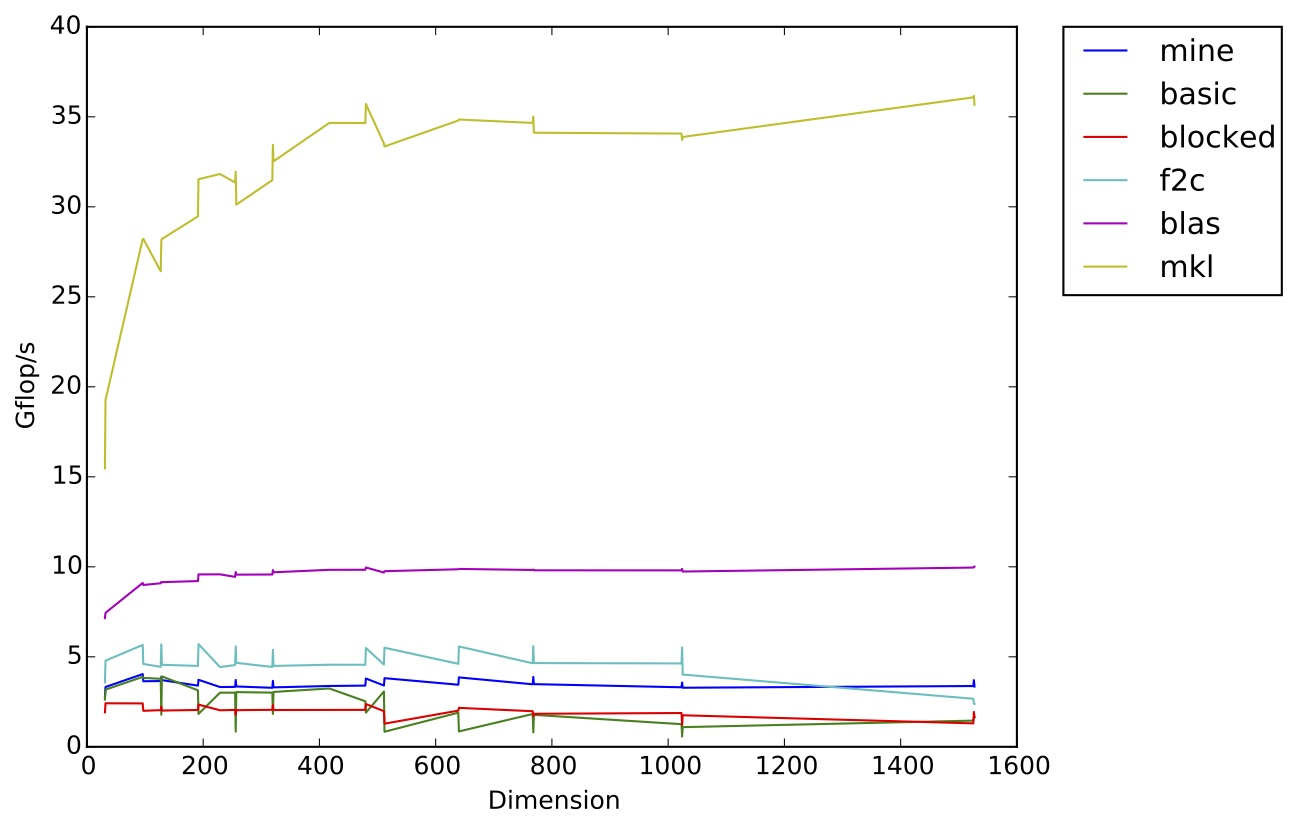
\includegraphics[width=0.8\textwidth]{cblocked_no_opt_flags}
    \caption{Blocked C matrix-matrix multiplication code with a blocked size of 512}
\end{figure}

\noindent It can be seen from Figure 1 that the blocking has helped stabilize the number of flop/s the program is able to do as the dimensions of the inputted matrices increase. Now this same blocking scheme is applied to a Fortran interfaced with C code, and the Fortran scheme is also taking advantage of allowing the strides taken in memory to be a minimum. The results can be found in Figure 2.

\begin{figure}[H]
  \centering
    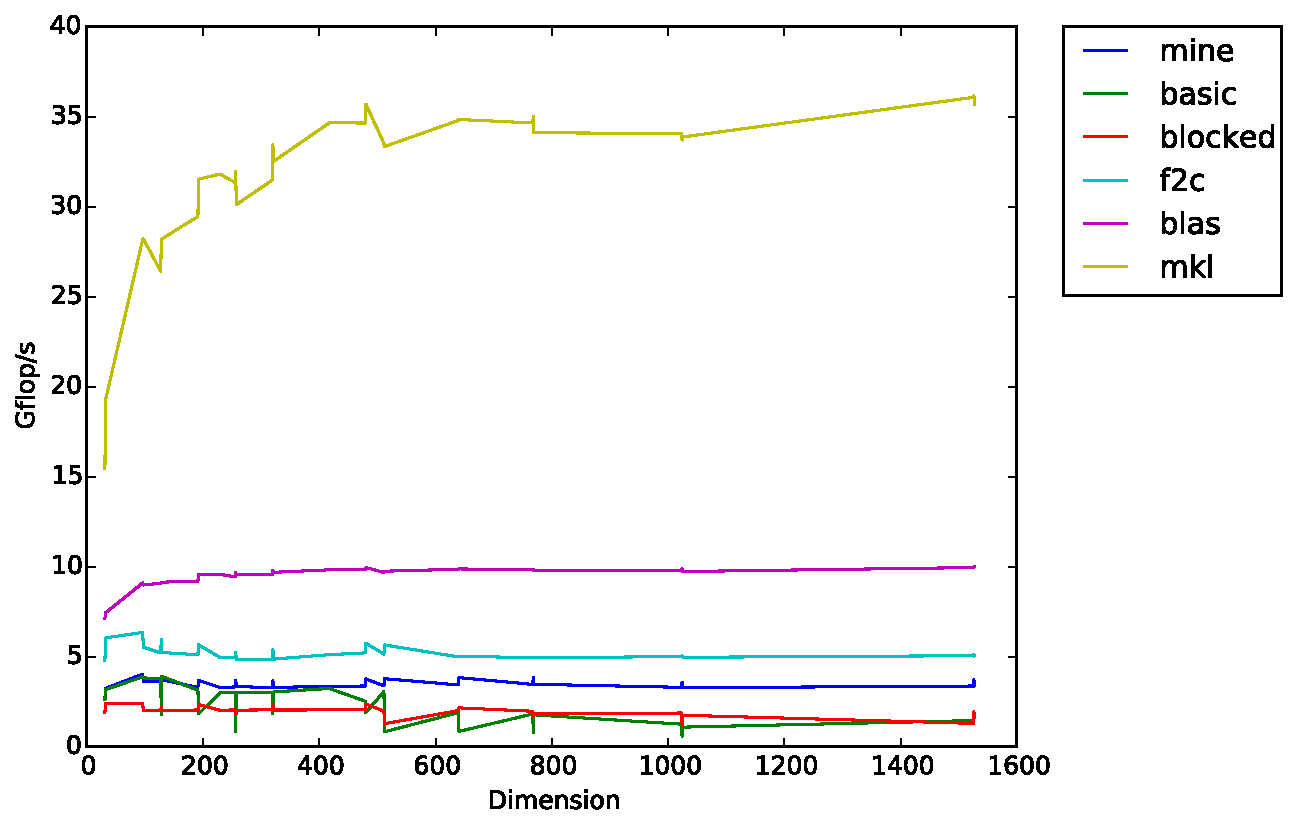
\includegraphics[width=0.8\textwidth]{c_f_blocked_no_opt_flags}
    \caption{Blocked C and Fortran matrix-matrix multiplication code with a blocked size of 512}
\end{figure}

\noindent While these results are an improvement over the naive approaches seen in the basic and blocked approaches, they are still only a fraction of the results obtained from the MKL and OpenBLAS libraries tuned to the server. It should be noted that the OpenBLAS results shown in Figures 1 and 2 are not using the optimized version.  Next, the optimized results that are using the following optimization flags:
\begin{verbatim}
-O3 -axcore-avx2 -mtune=core-avx2  -ftree-vectorize -funroll-loops -mtune=core-avx2
-xhost -ipo -no-prec-div -ansi-alias
\end{verbatim}
\noindent are introduced as well ensuring the block size being used will either fit into the L2 or L3 cache. This code also uses the most optimized form of code that takes advantage of the matrices layout in order to reduce the stride lengths taken. The results shown in Figures 3 use a block size of 380 which is a bit under the L3 cache size in order to accommodate for any other data that might end up being in the cache. The results shown in Figure 4 use a block size of 100 which is just under the L2 cache size for the same reasoning used in the L3 cache results. 

\begin{figure}[H]
  \centering
    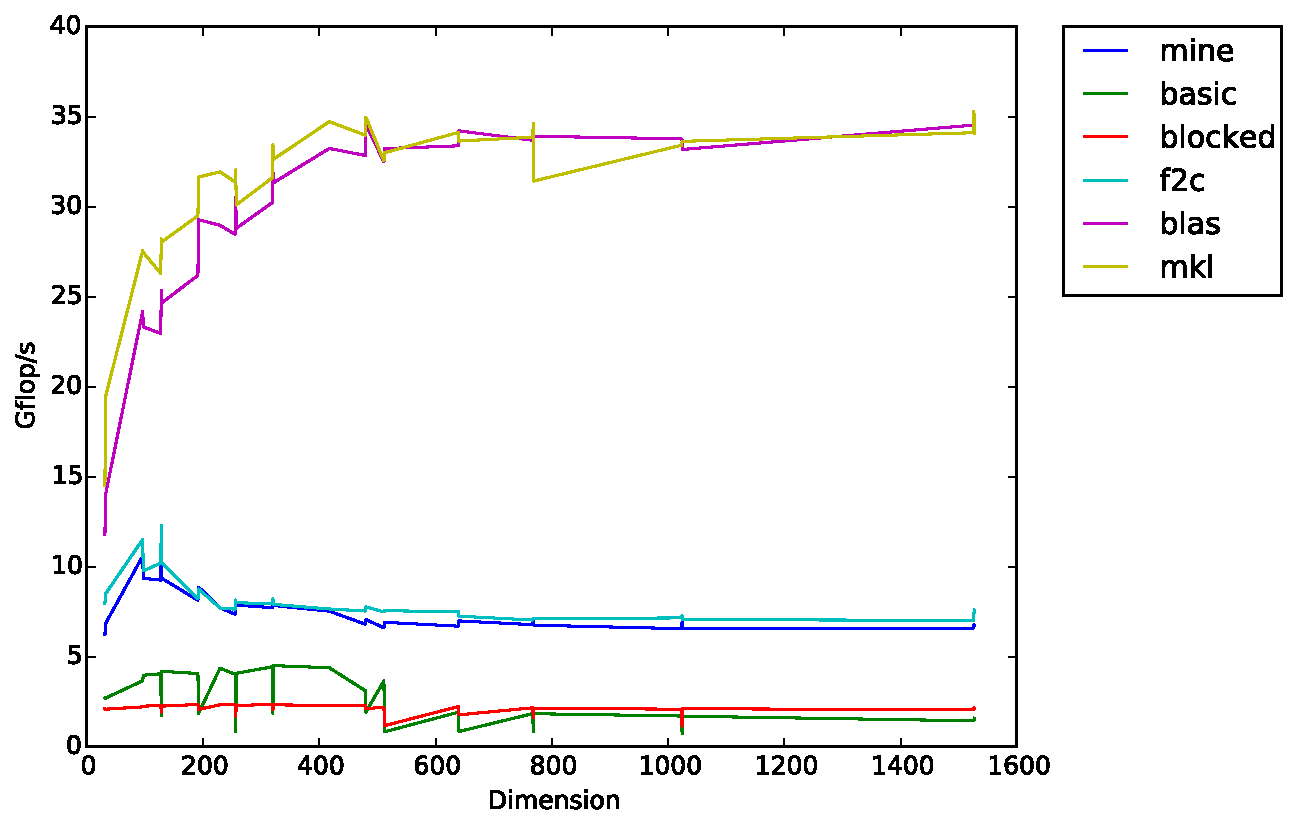
\includegraphics[width=0.8\textwidth]{c_f_blocked_opt_flags_b380}
    \caption{Optimized blocked C and Fortran matrix-matrix multiplication code with a blocked size of 380}
\end{figure}

\begin{figure}[H]
  \centering
    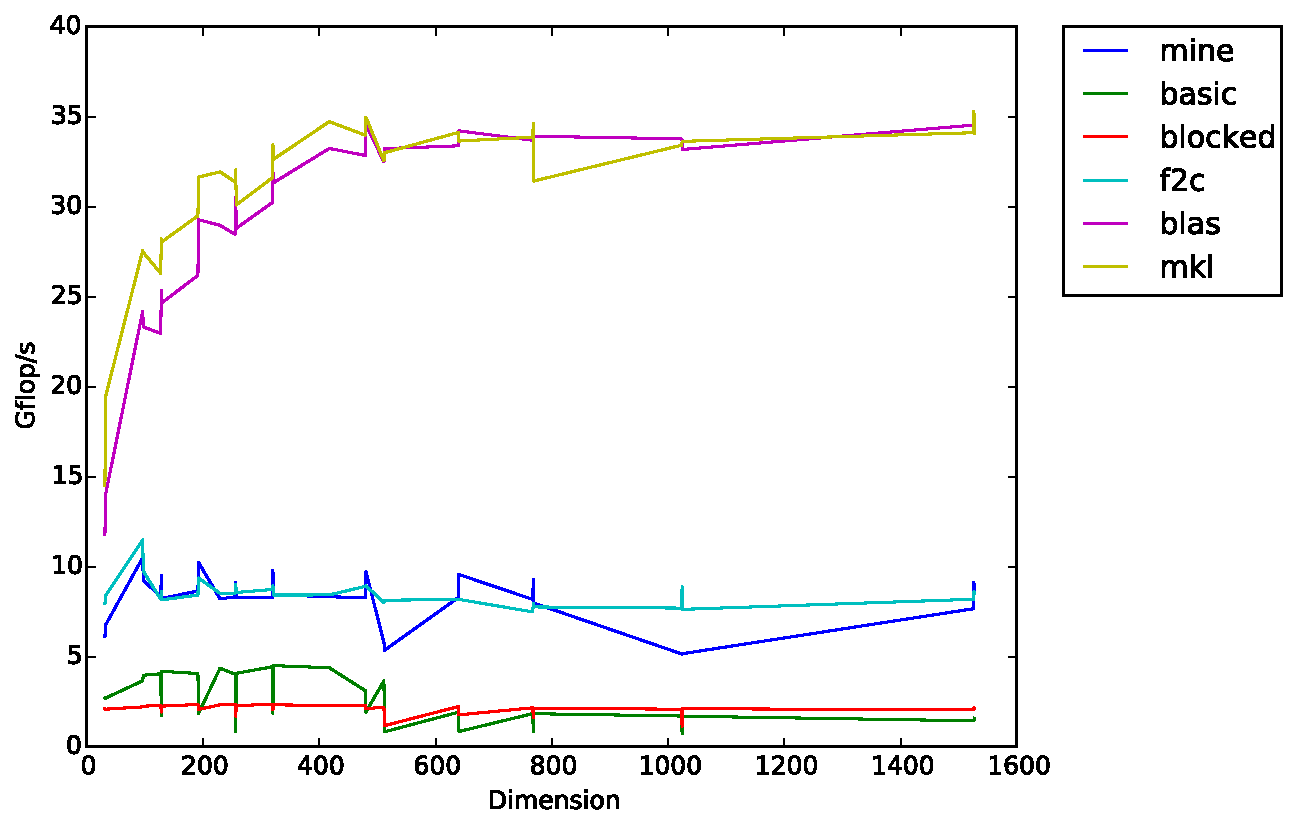
\includegraphics[width=0.8\textwidth]{c_f_blocked_opt_flags_b100}
    \caption{Optimized blocked C and Fortran matrix-matrix multiplication code with a blocked size of 100}
\end{figure}

\noindent  It should be noted that the optimized version of the OpenBLAS was used in the creation of these figures. Finally, these optimization flags were also applied to the naive Fortran code to see what results they have on it, and those can be found in Figure 5.

\begin{figure}[H]
  \centering
    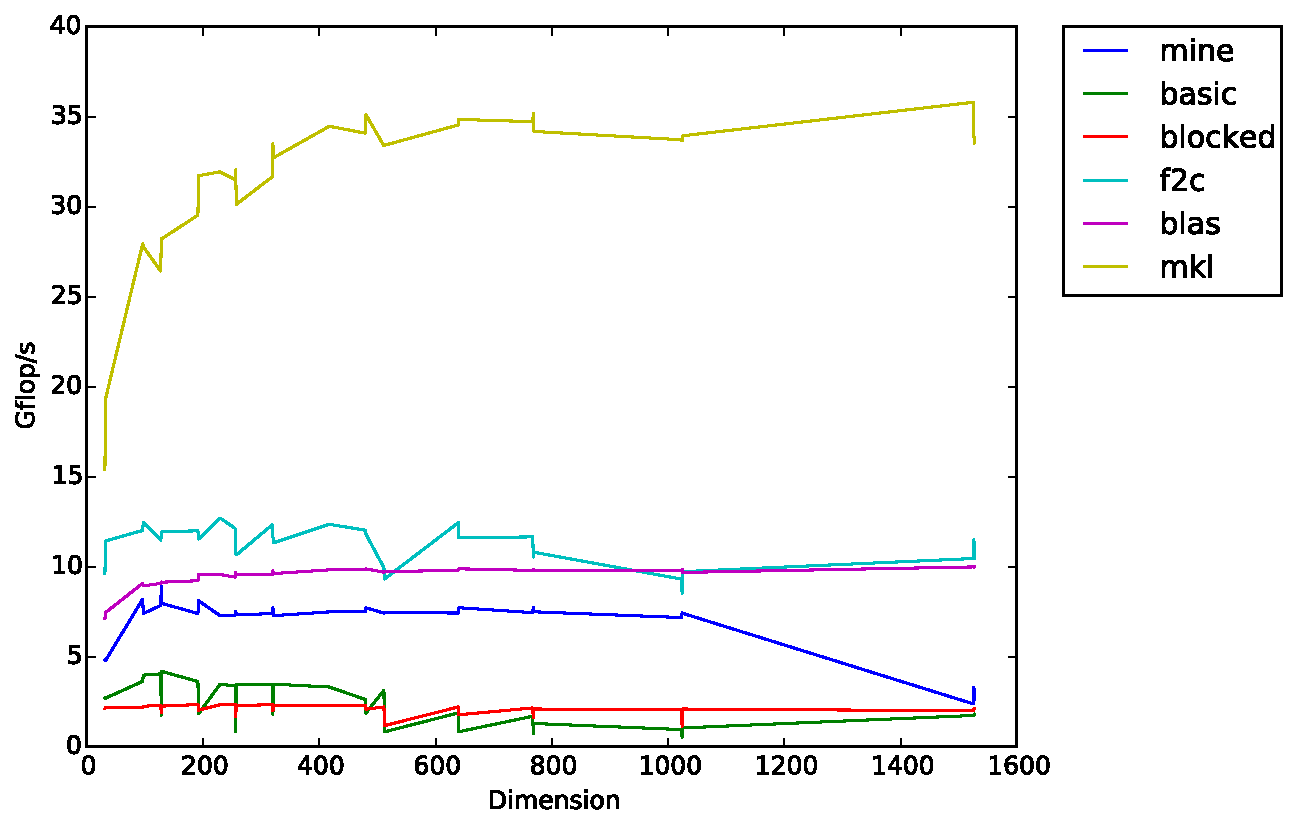
\includegraphics[width=0.8\textwidth]{naive_fortran_opt_flags}
    \caption{Naive Fortran code with optimization flags applied}
\end{figure}

\subsection{Advanced Hand Tuning:}

The results incorporating optimizations methods presented in the final optimization section along with using the appropriate loop layouts will be presented here. First, the Fortran program results will be shown in Figure 6:

\begin{figure}[H]
  \centering
    \includegraphics[width=0.8\textwidth]{fortranevolution}
    \caption{Evolution of Fortran program speed-ups when incorporating different optimization methods}
\end{figure}

\noindent Several different results can be seen in Figure 6. The biggest one to note when comparing Figure 6 to Figure 1 is that the optimization flags supplied by the compiler have a huge effect on increasing the performance of the code. Next, it can be seen that the multi-blocking scheme leads to several sharp drops every time a new block has to be introduced at the L2 cache level. Based on the above chart, it can be seen that the vectorized fortran code with L2 blocks of 96 and L1 blocks of 32, labeled fortran\_blocked\_L2\_96\_blocked\_L1\_32 in Figure 6, is the highest performing where it ultimately ends up performing just ever so slightly better than the non optimized BLAS implementation. It should also be noted the difference between that code and the non vectorized version as fortran\_2\_level\_blocked\_non\_vectorized in Figure 6. The vectorized code provides a significant boost in performance. Next, the results from the C program results will be shown in Figure 7.

\begin{figure}[H]
  \centering
    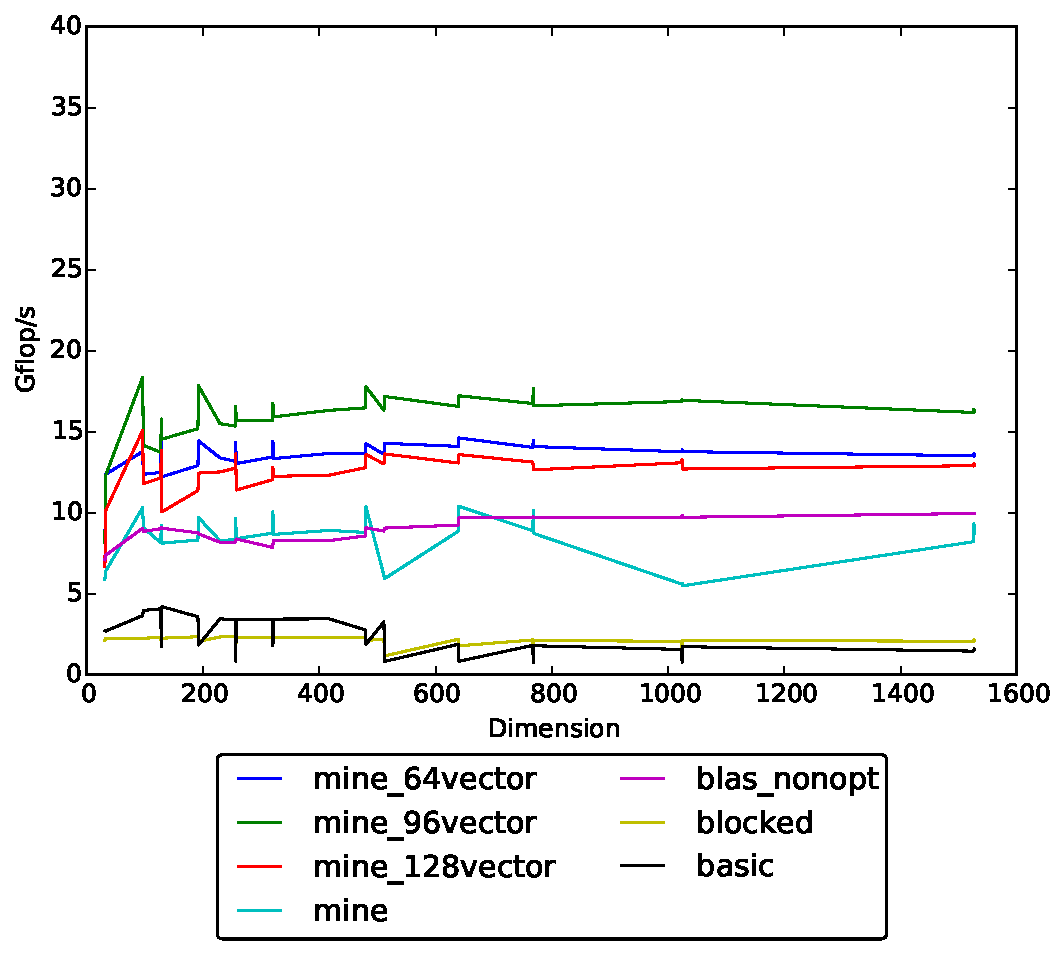
\includegraphics[width=0.8\textwidth]{cevolution}
    \caption{Evolution of C program speed-ups when incorporating different optimization methods}
\end{figure}

\noindent The copy optimized and vectorized versions of the matrix-matrix multiply implementations can be seen to have a large improvement over the simple optimized blocked version as noted as "mine" in Figure 7. Then it can also be seen that the optimized C code performs amazingly well when compared to the initial naive implementations. It can also be noted that the best performing version of the code can be found when the block sized used is 96x96 in the vectorized version of the code. It can also be noted that all of the vectorized versions of the C program out perform the non optimized BLAS code which is quite impressive. Now the final optimized programs will be shown against all MKL, optimized BLAS, and the other implementations already noted.

\begin{figure}[H]
  \centering
    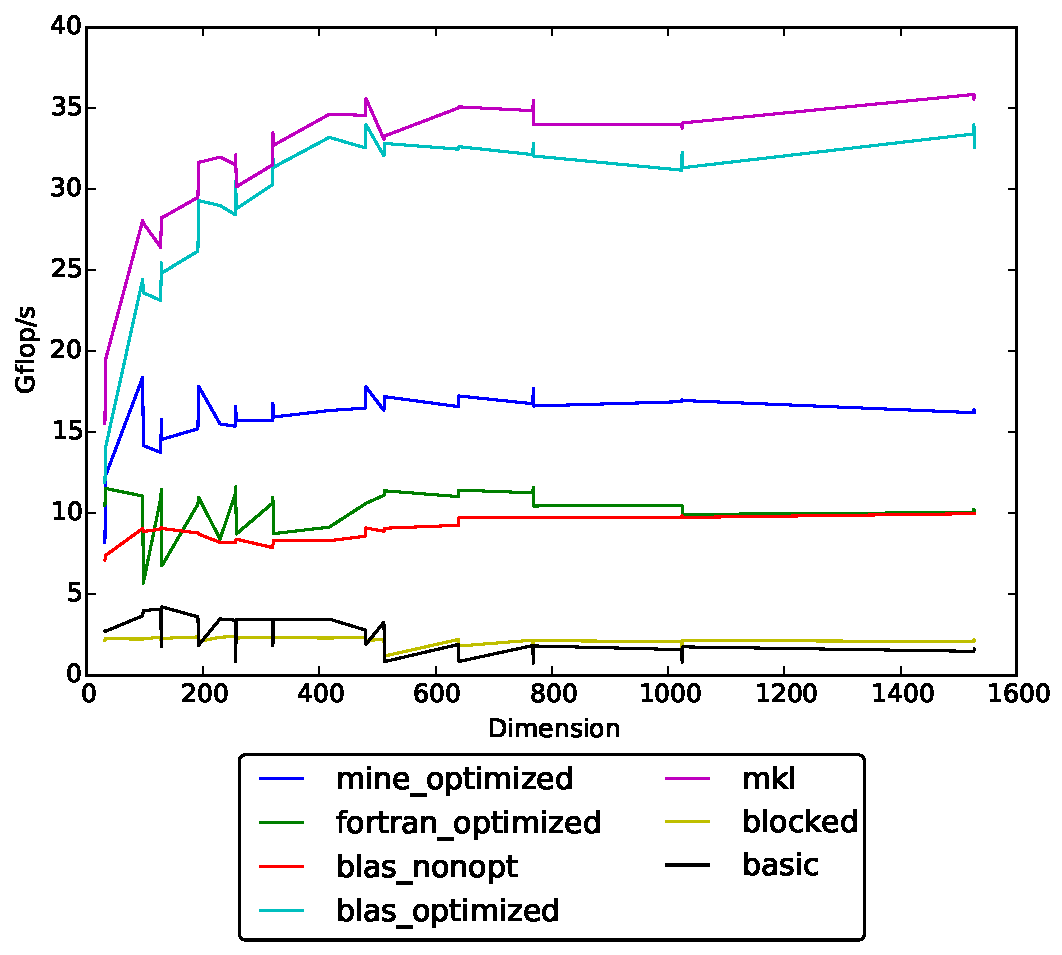
\includegraphics[width=0.8\textwidth]{timing-optimized}
    \caption{Final optimized C and Fortran programs when incorporating different optimization methods}
\end{figure}

\noindent The first thing to note from this figure is that both final optimized codes beat the non optimized BLAS code. Yet, they still can't reach the same levels as the optimized matrix libraries already built. Next, it should be noted that the C program reaches 45\% of the MKL performance a very impressive result. It also beats out the optimized Fortran code which strongly contradicts what the initial results would have suggested about C's ability to perform against Fortran. 

\section*{Analysis:}

Several tuning methods were shown to work fairly well in improving the performance of the matrix-matrix multiplication. The use of optimization flags had by far the largest effect on improving the performance of the code. Although, if the wrong flags were used then a performance degradation could occur or one less efficient flag could supersede the use of a more efficient flag. For example, if the ftree-vectorize and axcore-avx2 flags are both used the ftree-vectorize flag will be used even though the axcore-avx2 flag allows for better performance.  Next, the blocking worked in that it stabilized the calculations in most cases and resulted in fairly "constant" performance as the size of the matrix increased. The vectorization also provided a large improvement in the performance of the code by allowing the program to become less bandwidth limited. The multi-level blocking scheme had mixed results when using Fortran it was seen to have a beneficial performance boost, while the C program had the opposite effect where it degraded the performance.  Several improvements could still be made to both codes by examining the use of fast kernel matrix-matrix multiply operations that take direct advantage of the AVX2 instruction set. So, they wouldn't be based upon the automatic vectorization that the compiler performs. It would most likely be easier in C to perform this than Fortran, since Intel provides more low-level options for the AVX2 instruction set in C/C++ than in Fortran. Overall, one can obtain fairly high performing matrix-matrix multiplications, but they would be better off using either MKL or an optimized BLAS implementation due to the higher obtained performance.

\section*{References:}

\noindent [1] https://software.intel.com/en-us/node/579324 \\ \\
\noindent [2] https://software.intel.com/en-us/node/579297 \\ \\
\noindent [3] https://software.intel.com/en-us/node/579313 \\ \\
\noindent [4] https://software.intel.com/en-us/node/579421 \\ \\
\noindent [5]  https://gcc.gnu.org/onlinedocs/gcc/Optimize-Options.html\#Optimize-Options \\  \\


\end{document}